\section{Results}
\label{sec:results}

To proceed into the experiments, the methodology of test will have the trained models, DQN and RL, perform a series of test between alternating the competitive selection between the variable the normal best, and then the specific competitive variable, and the same
competitive variable without alternation per trained model. This was by playing 50 episodes/games against each opponent, for example a DQN with alternating and neutral competitive versus a normal DQN, QL, or random. To provide a baseline of which is better, DQN or 
QL in this situation based on the training they received, the below chart are those two head to head.

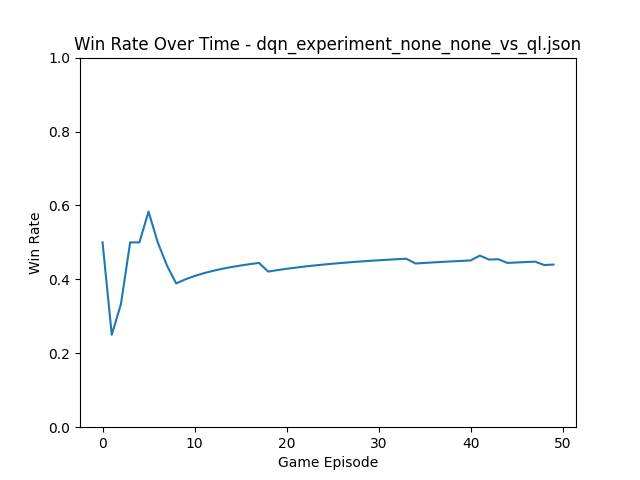
\includegraphics[width=0.5\textwidth]{images/win_rate_dqn_experiment_none_none_vs_ql.png}

From this baseline it can be seen that the DQN and the QL model perform around the same level, and looking into the statistics themselves of their competition nearly every game was a stalemate with only a few games where one conquered the other. 

\subsection{Data}

To clarify what the below charts mean by win rate, a win consists of a 1, a loss, 0, but since a tie in essence is also an desirable state considering that would mean it is challenging enough to not lose, but scales to the difficulty to not win as well, a tie
adds .5 to the win ratio, meaning that if a model tied every single game it would achieve a desirable 50 percent win ratio. This does slightly skew the results due to that caveat but the results it produces are beneficial for this experiment specifically. 
In addition, there is more information available that includes total rewards and a moving average reward included in the Appendix A, but for the sake of readability it was not included here.

\begin{tabular}{>{\centering\arraybackslash}m{0.05\textwidth}>{\centering\arraybackslash}m{0.3\textwidth}>{\centering\arraybackslash}m{0.25\textwidth}>{\centering\arraybackslash}m{0.25\textwidth}}
    & \multicolumn{3}{c}{\textbf{DQN without Alternating}} \\
    & \textbf{Vs Random} & \textbf{Vs QL} & \textbf{Vs DQN} \\
    \textbf{Neutral} & 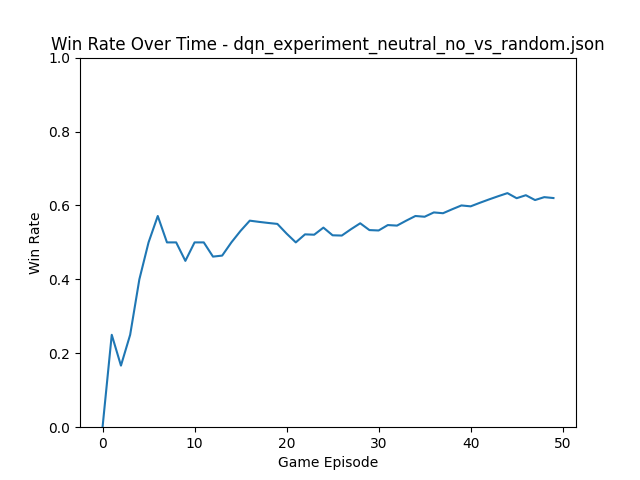
\includegraphics[width=0.25\textwidth]{images/win_rate_dqn_experiment_neutral_no_vs_random.png} &
    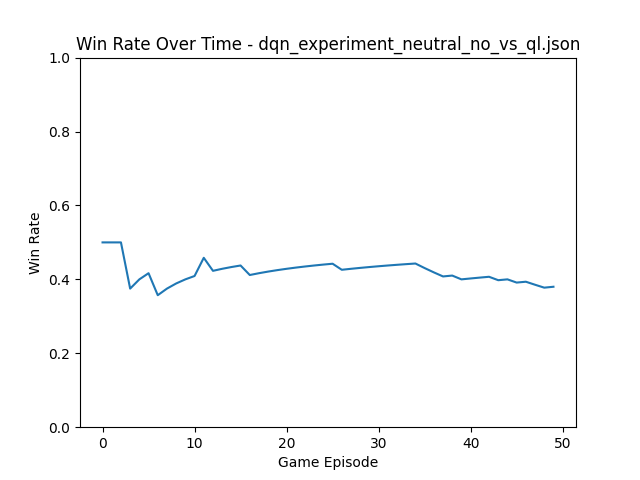
\includegraphics[width=0.25\textwidth]{images/win_rate_dqn_experiment_neutral_no_vs_ql.png} &
    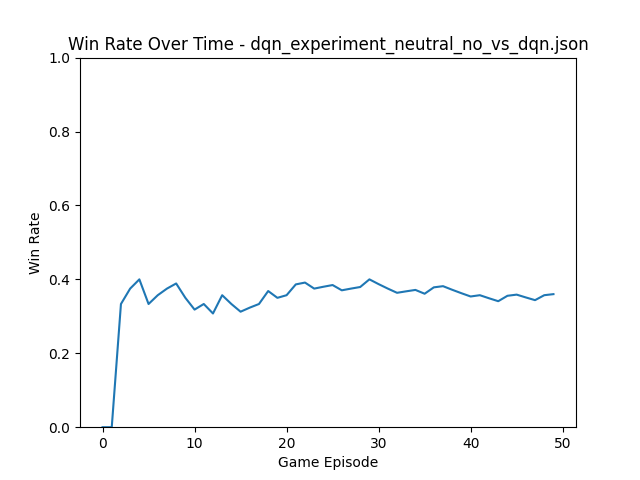
\includegraphics[width=0.25\textwidth]{images/win_rate_dqn_experiment_neutral_no_vs_dqn.png} \\
    \textbf{Half} &  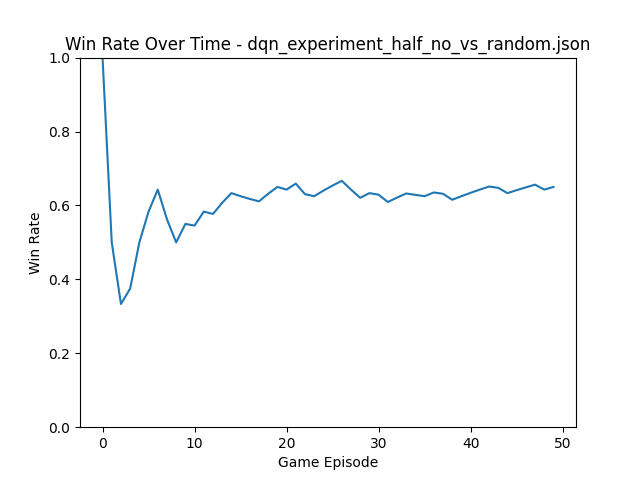
\includegraphics[width=0.25\textwidth]{images/win_rate_dqn_experiment_half_no_vs_random.png} & 
    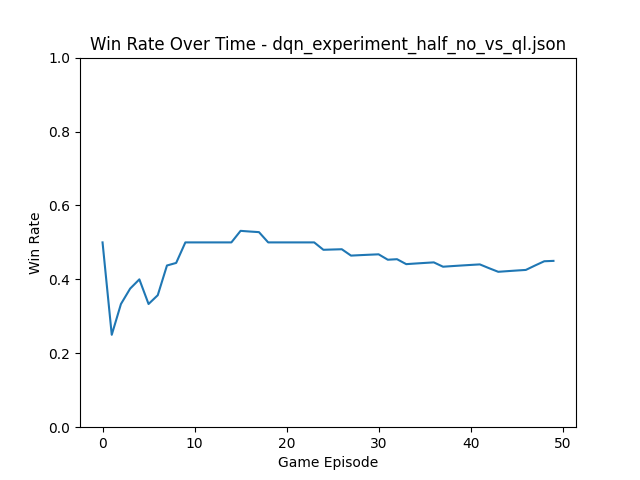
\includegraphics[width=0.25\textwidth]{images/win_rate_dqn_experiment_half_no_vs_ql.png} &
    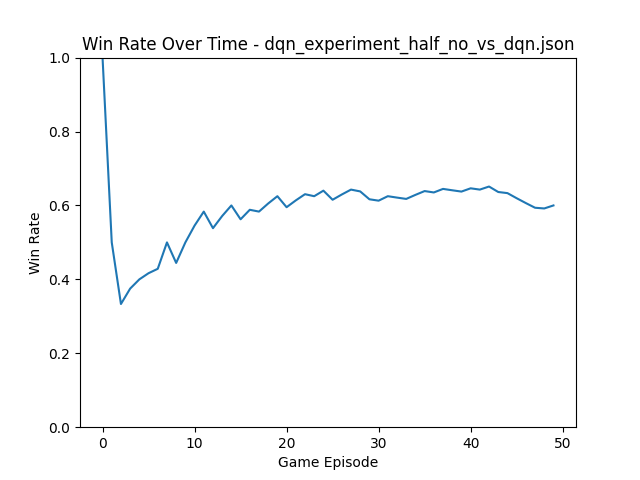
\includegraphics[width=0.25\textwidth]{images/win_rate_dqn_experiment_half_no_vs_dqn.png} \\
    \textbf{Quarter} & 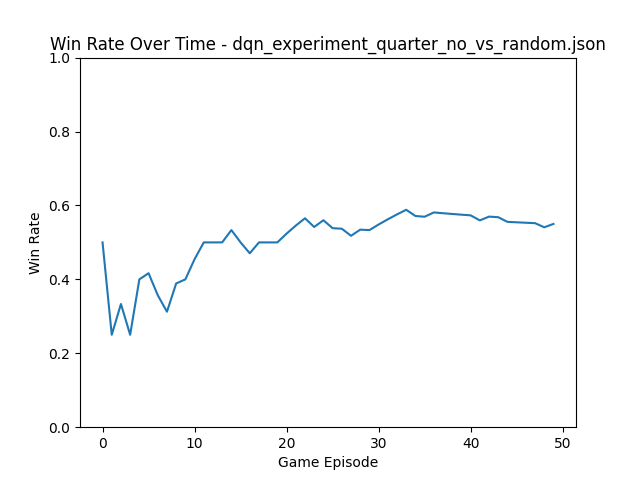
\includegraphics[width=0.25\textwidth]{images/win_rate_dqn_experiment_quarter_no_vs_random.png} &
    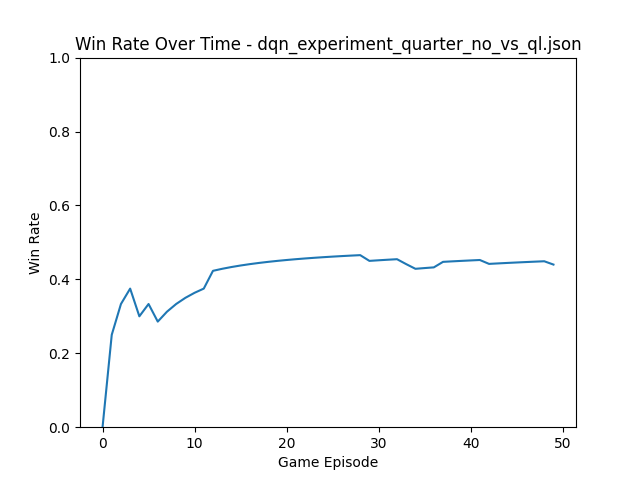
\includegraphics[width=0.25\textwidth]{images/win_rate_dqn_experiment_quarter_no_vs_ql.png} &
    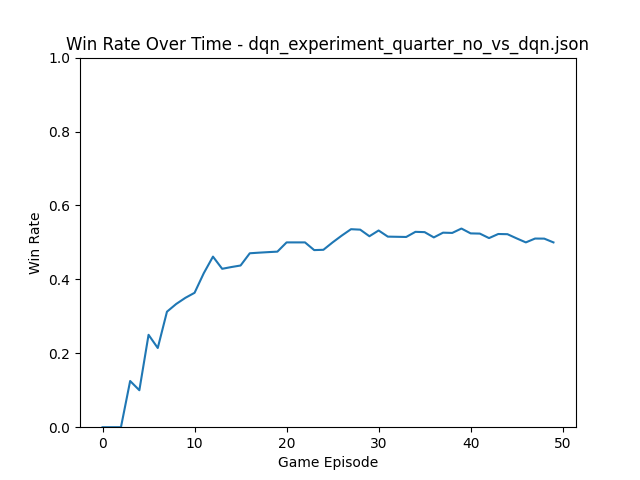
\includegraphics[width=0.25\textwidth]{images/win_rate_dqn_experiment_quarter_no_vs_dqn.png} \\
    \textbf{Second} & 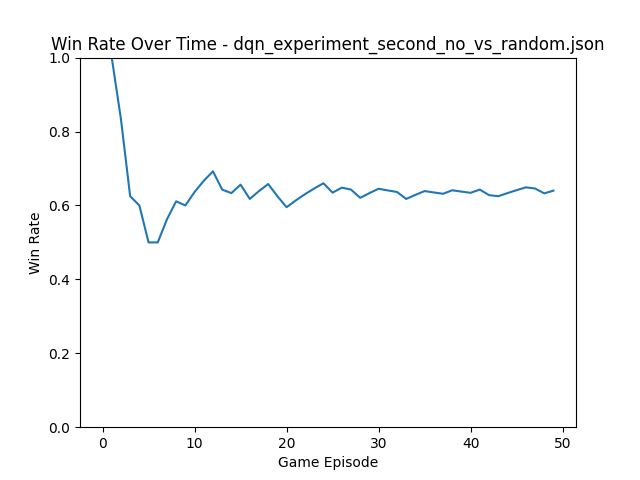
\includegraphics[width=0.25\textwidth]{images/win_rate_dqn_experiment_second_no_vs_random.png} &
    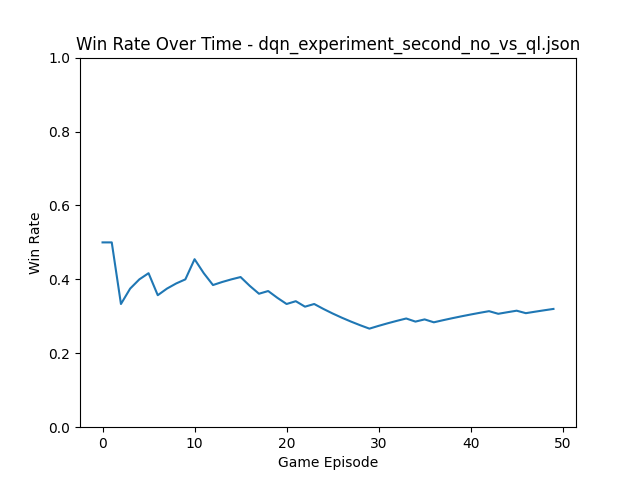
\includegraphics[width=0.25\textwidth]{images/win_rate_dqn_experiment_second_no_vs_ql.png} &
    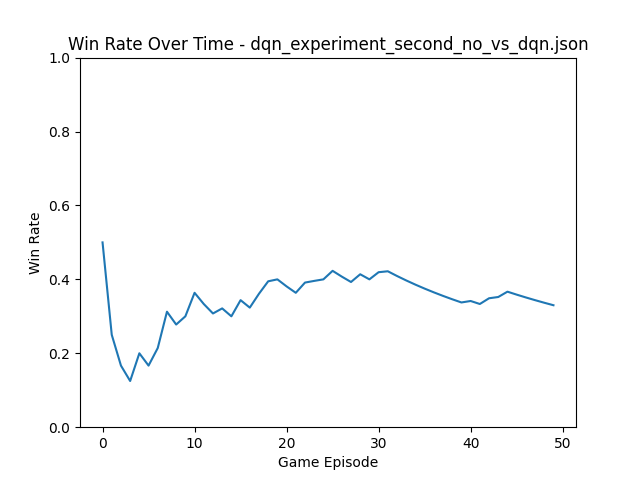
\includegraphics[width=0.25\textwidth]{images/win_rate_dqn_experiment_second_no_vs_dqn.png} \\
  \end{tabular}

  \begin{tabular}{>{\centering\arraybackslash}m{0.05\textwidth}>{\centering\arraybackslash}m{0.3\textwidth}>{\centering\arraybackslash}m{0.25\textwidth}>{\centering\arraybackslash}m{0.25\textwidth}}
    & \multicolumn{3}{c}{\textbf{DQN with Alternating}} \\
    & \textbf{Vs Random} & \textbf{Vs QL} & \textbf{Vs DQN} \\
    \textbf{Neutral} & 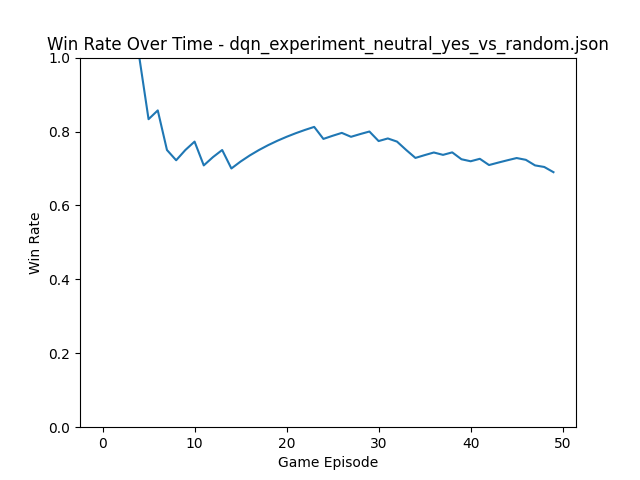
\includegraphics[width=0.25\textwidth]{images/win_rate_dqn_experiment_neutral_yes_vs_random.png} &
    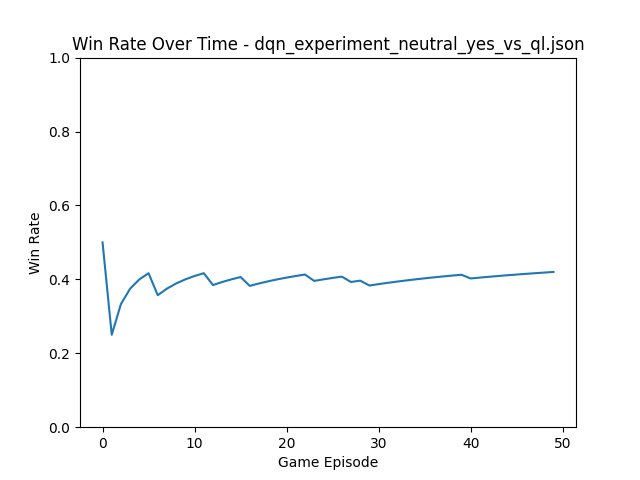
\includegraphics[width=0.25\textwidth]{images/win_rate_dqn_experiment_neutral_yes_vs_ql.png} &
    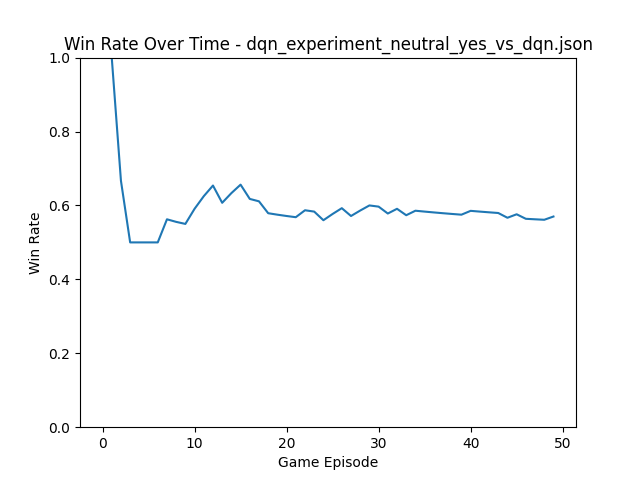
\includegraphics[width=0.25\textwidth]{images/win_rate_dqn_experiment_neutral_yes_vs_dqn.png} \\
    \textbf{Half} &  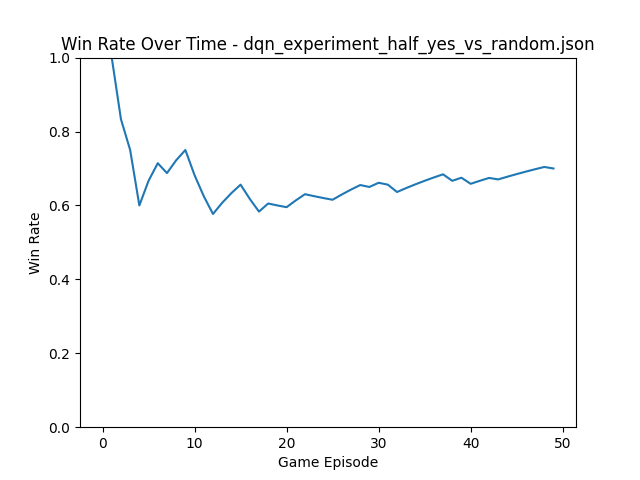
\includegraphics[width=0.25\textwidth]{images/win_rate_dqn_experiment_half_yes_vs_random.png} & 
    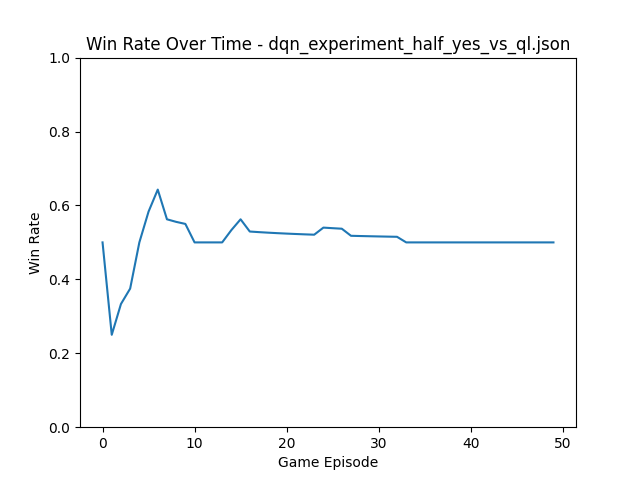
\includegraphics[width=0.25\textwidth]{images/win_rate_dqn_experiment_half_yes_vs_ql.png} &
    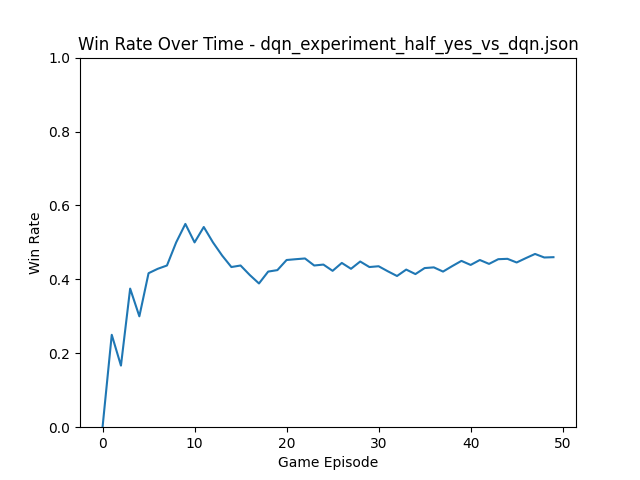
\includegraphics[width=0.25\textwidth]{images/win_rate_dqn_experiment_half_yes_vs_dqn.png} \\
    \textbf{Quarter} & 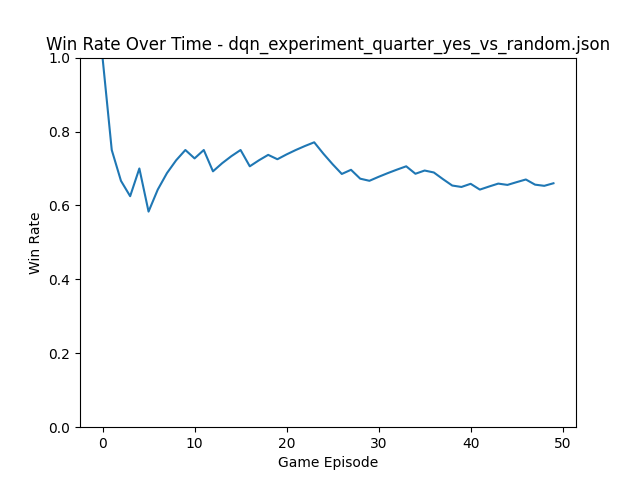
\includegraphics[width=0.25\textwidth]{images/win_rate_dqn_experiment_quarter_yes_vs_random.png} &
    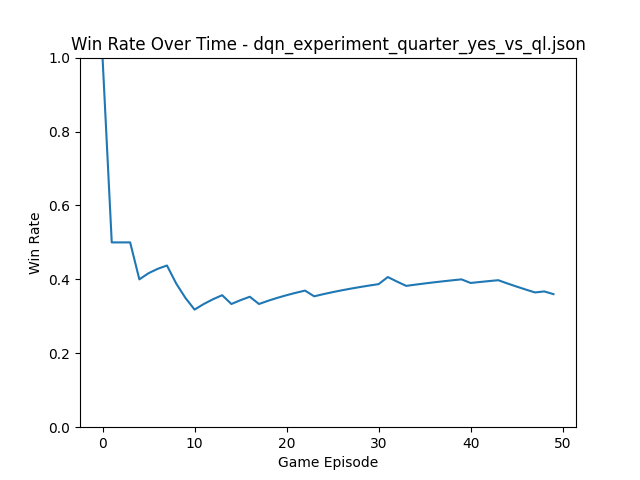
\includegraphics[width=0.25\textwidth]{images/win_rate_dqn_experiment_quarter_yes_vs_ql.png} &
    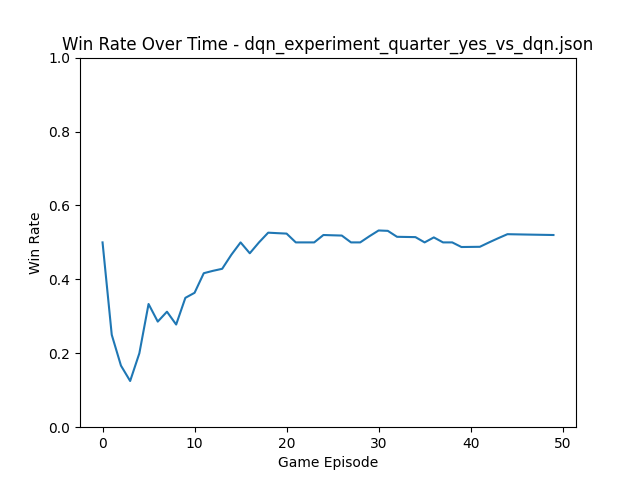
\includegraphics[width=0.25\textwidth]{images/win_rate_dqn_experiment_quarter_yes_vs_dqn.png} \\
    \textbf{Second} & 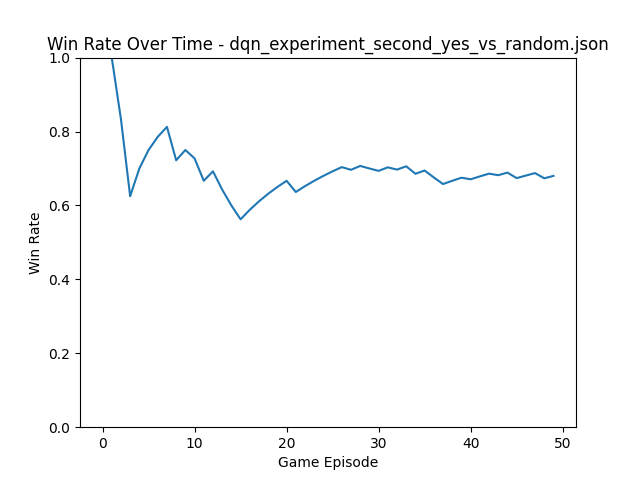
\includegraphics[width=0.25\textwidth]{images/win_rate_dqn_experiment_second_yes_vs_random.png} &
    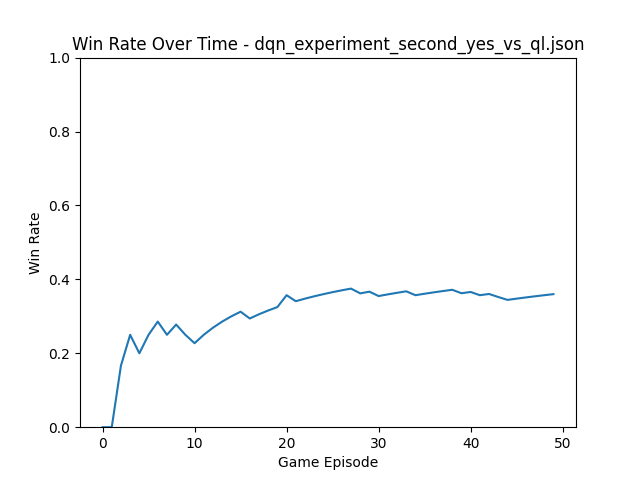
\includegraphics[width=0.25\textwidth]{images/win_rate_dqn_experiment_second_yes_vs_ql.png} &
    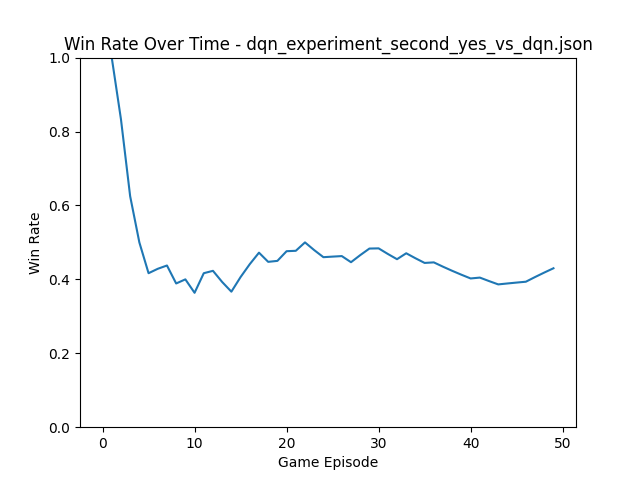
\includegraphics[width=0.25\textwidth]{images/win_rate_dqn_experiment_second_yes_vs_dqn.png} \\
  \end{tabular}

  \begin{tabular}{>{\centering\arraybackslash}m{0.05\textwidth}>{\centering\arraybackslash}m{0.3\textwidth}>{\centering\arraybackslash}m{0.25\textwidth}>{\centering\arraybackslash}m{0.25\textwidth}}
    & \multicolumn{3}{c}{\textbf{QL without Alternating}} \\
    & \textbf{Vs Random} & \textbf{Vs QL} & \textbf{Vs DQN} \\
    \textbf{Neutral} & 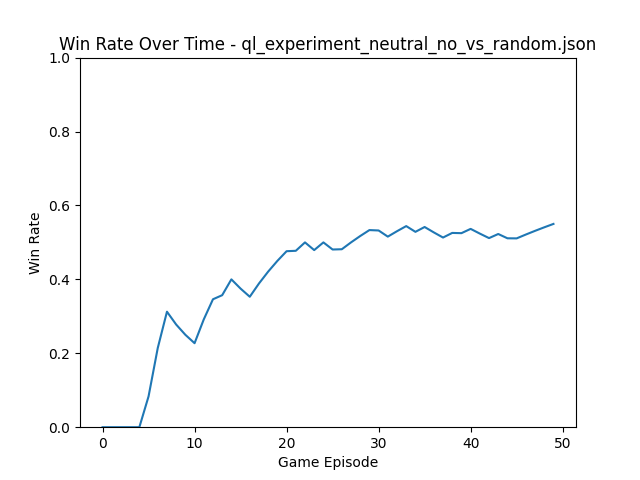
\includegraphics[width=0.25\textwidth]{images/win_rate_ql_experiment_neutral_no_vs_random.png} &
    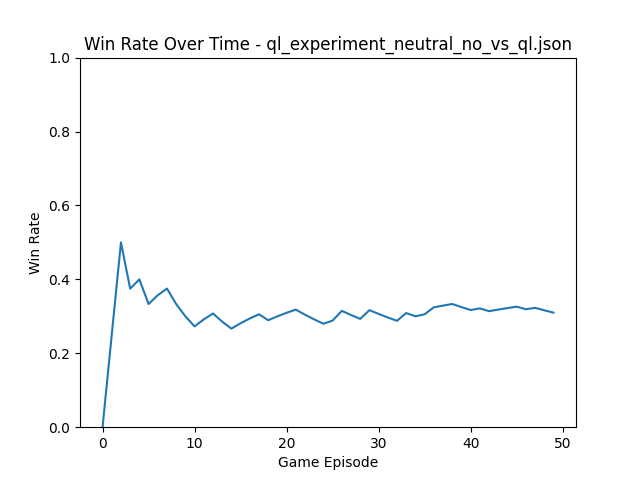
\includegraphics[width=0.25\textwidth]{images/win_rate_ql_experiment_neutral_no_vs_ql.png} &
    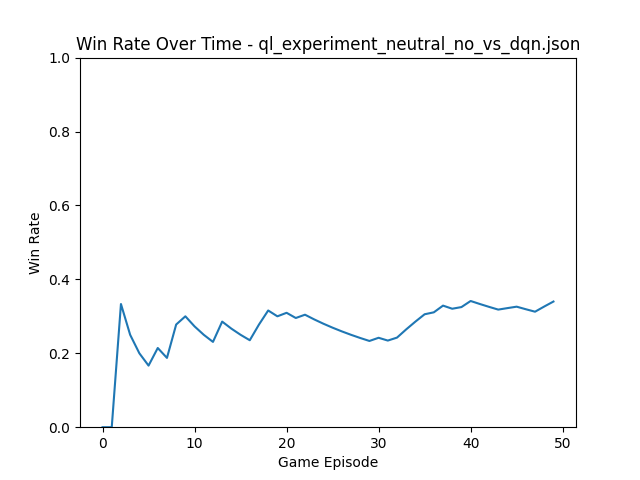
\includegraphics[width=0.25\textwidth]{images/win_rate_ql_experiment_neutral_no_vs_dqn.png} \\
    \textbf{Half} &  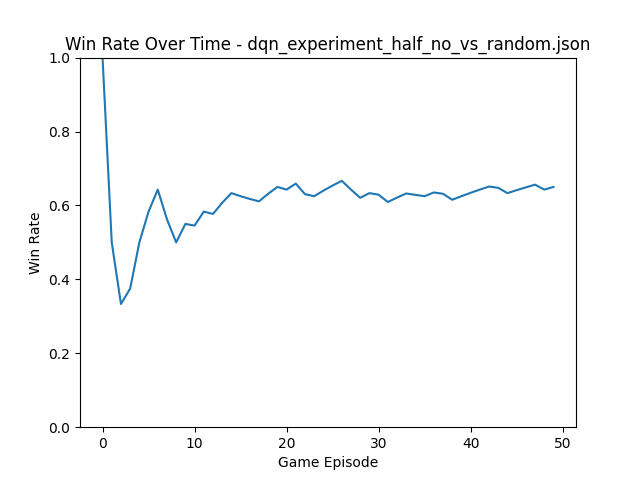
\includegraphics[width=0.25\textwidth]{images/win_rate_dqn_experiment_half_no_vs_random.png} & 
    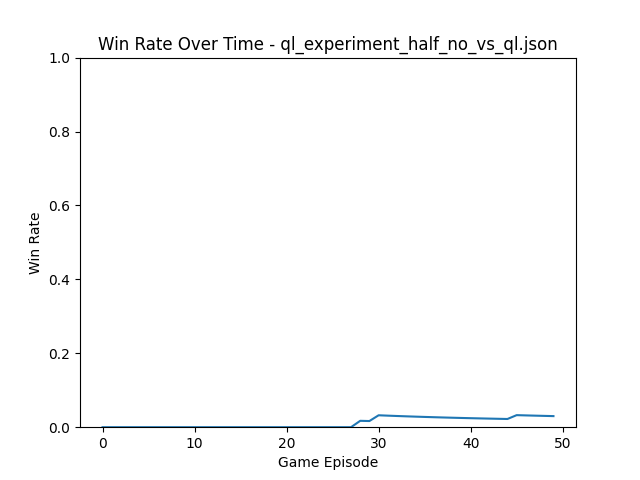
\includegraphics[width=0.25\textwidth]{images/win_rate_ql_experiment_half_no_vs_ql.png} &
    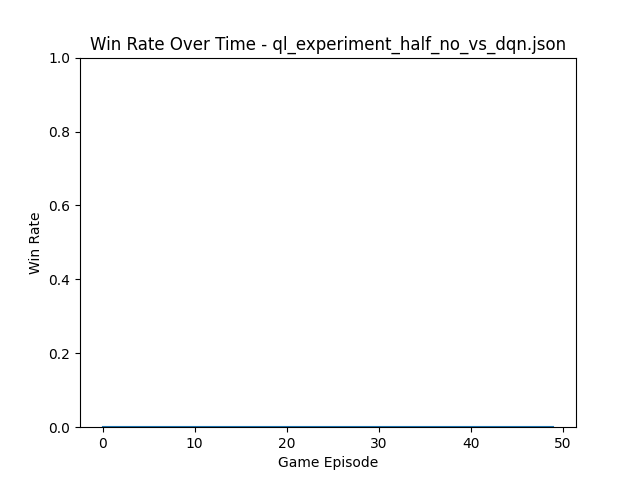
\includegraphics[width=0.25\textwidth]{images/win_rate_ql_experiment_half_no_vs_dqn.png} \\
    \textbf{Quarter} & 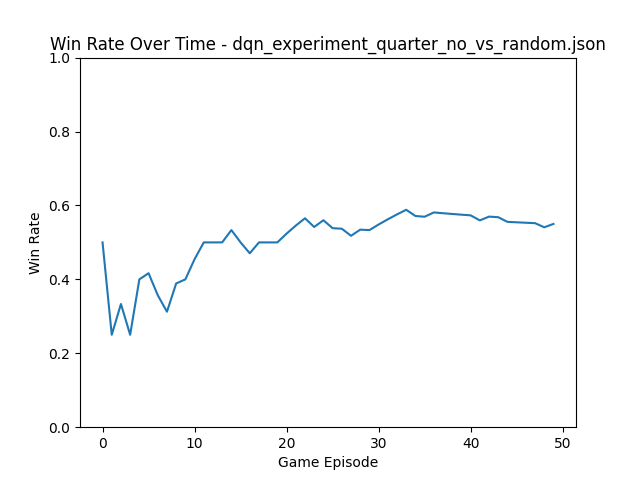
\includegraphics[width=0.25\textwidth]{images/win_rate_dqn_experiment_quarter_no_vs_random.png} &
    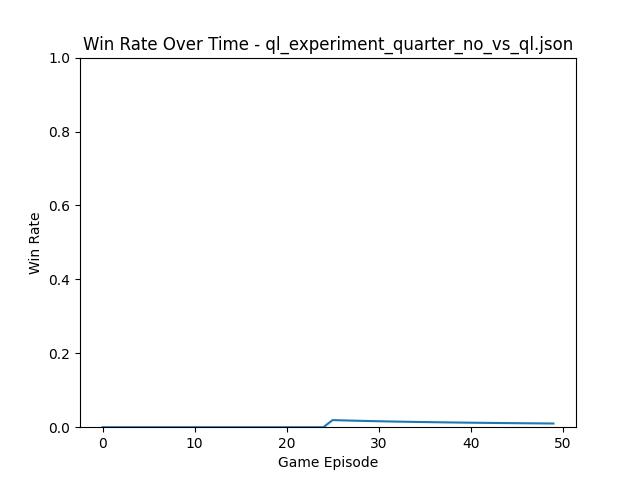
\includegraphics[width=0.25\textwidth]{images/win_rate_ql_experiment_quarter_no_vs_ql.png} &
    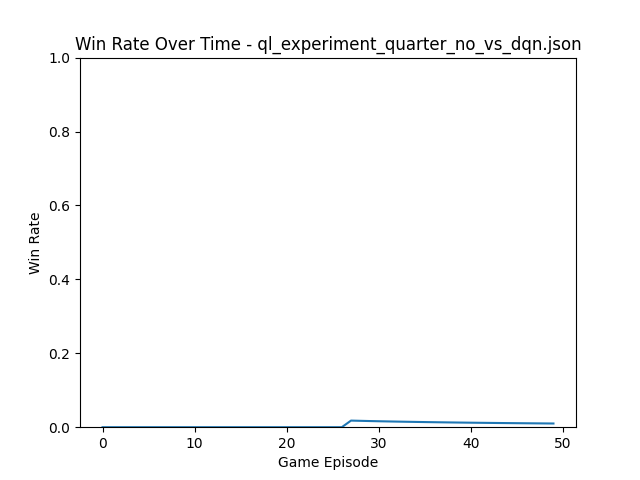
\includegraphics[width=0.25\textwidth]{images/win_rate_ql_experiment_quarter_no_vs_dqn.png} \\
    \textbf{Second} & 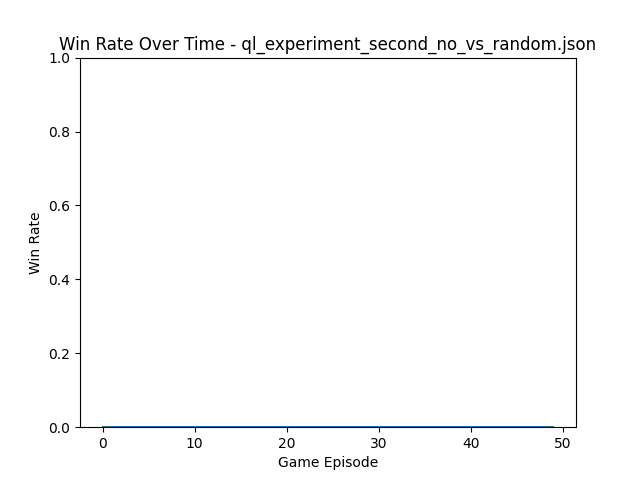
\includegraphics[width=0.25\textwidth]{images/win_rate_ql_experiment_second_no_vs_random.png} &
    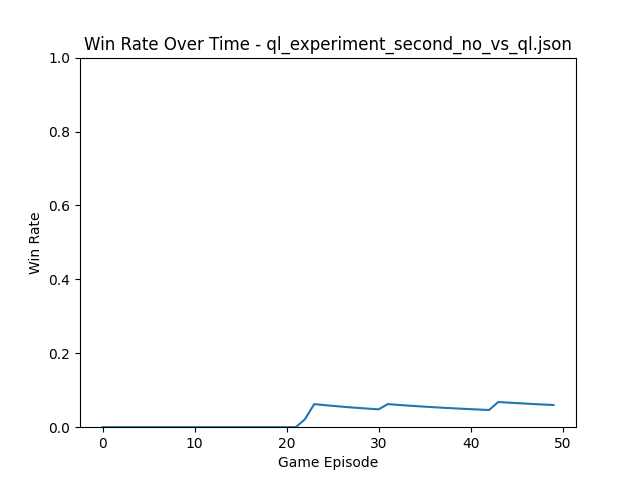
\includegraphics[width=0.25\textwidth]{images/win_rate_ql_experiment_second_no_vs_ql.png} &
    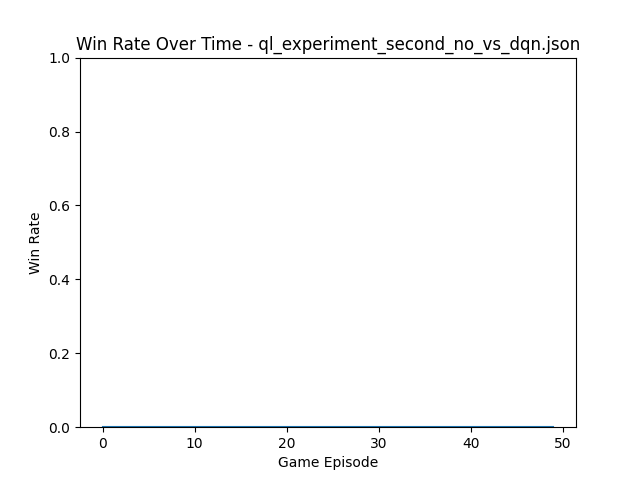
\includegraphics[width=0.25\textwidth]{images/win_rate_ql_experiment_second_no_vs_dqn.png} \\
  \end{tabular}

  \begin{tabular}{>{\centering\arraybackslash}m{0.05\textwidth}>{\centering\arraybackslash}m{0.3\textwidth}>{\centering\arraybackslash}m{0.25\textwidth}>{\centering\arraybackslash}m{0.25\textwidth}}
    & \multicolumn{3}{c}{\textbf{QL with Alternating}} \\
    & \textbf{Vs Random} & \textbf{Vs QL} & \textbf{Vs DQN} \\
    \textbf{Neutral} & 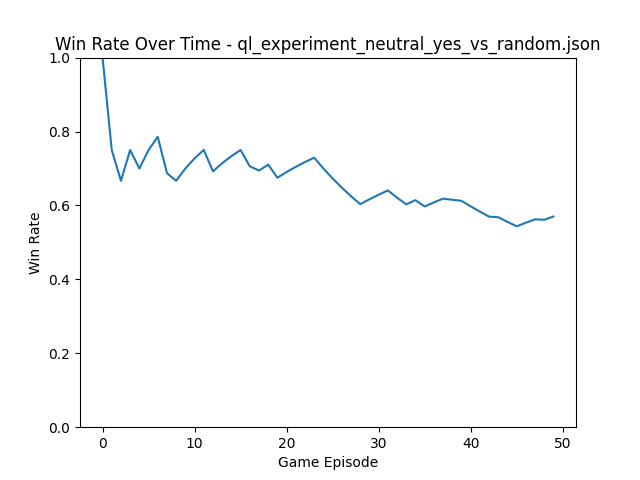
\includegraphics[width=0.25\textwidth]{images/win_rate_ql_experiment_neutral_yes_vs_random.png} &
    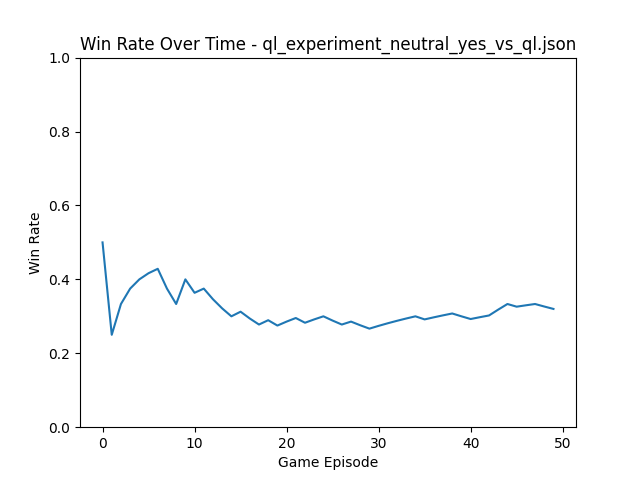
\includegraphics[width=0.25\textwidth]{images/win_rate_ql_experiment_neutral_yes_vs_ql.png} &
    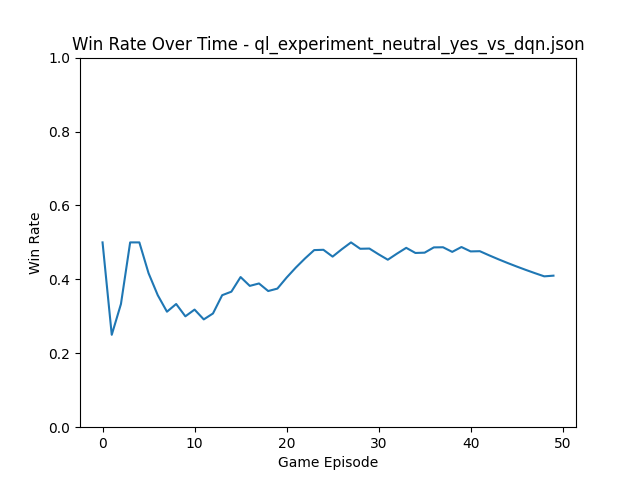
\includegraphics[width=0.25\textwidth]{images/win_rate_ql_experiment_neutral_yes_vs_dqn.png} \\
    \textbf{Half} &  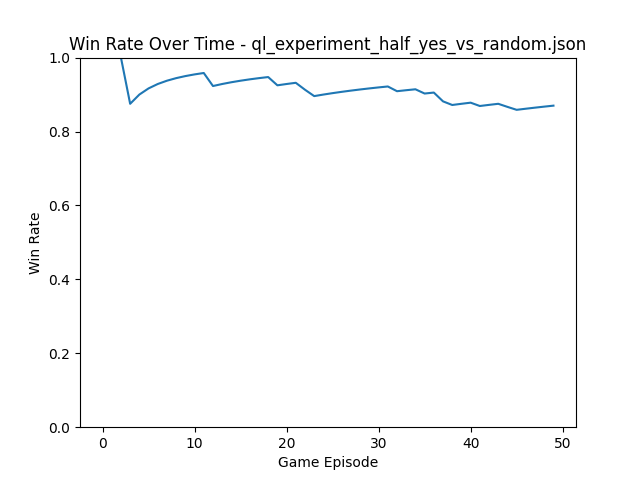
\includegraphics[width=0.25\textwidth]{images/win_rate_ql_experiment_half_yes_vs_random.png} & 
    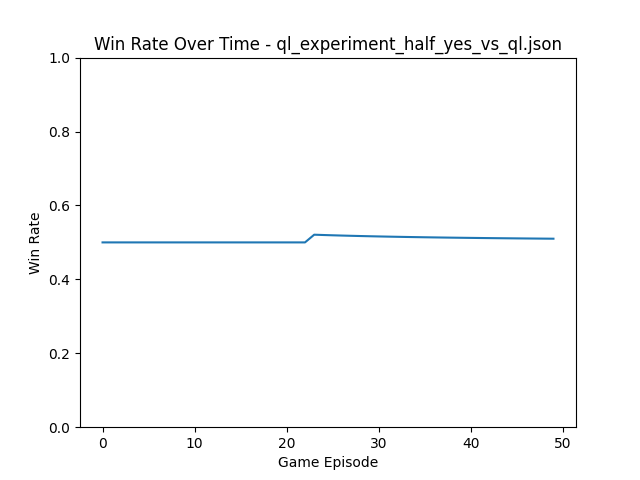
\includegraphics[width=0.25\textwidth]{images/win_rate_ql_experiment_half_yes_vs_ql.png} &
    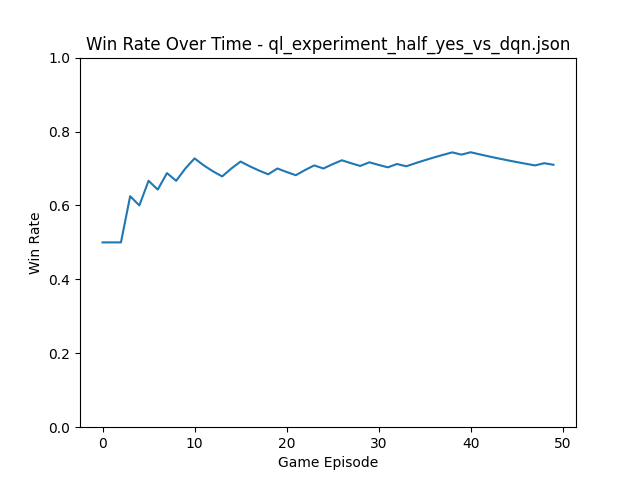
\includegraphics[width=0.25\textwidth]{images/win_rate_ql_experiment_half_yes_vs_dqn.png} \\
    \textbf{Quarter} & 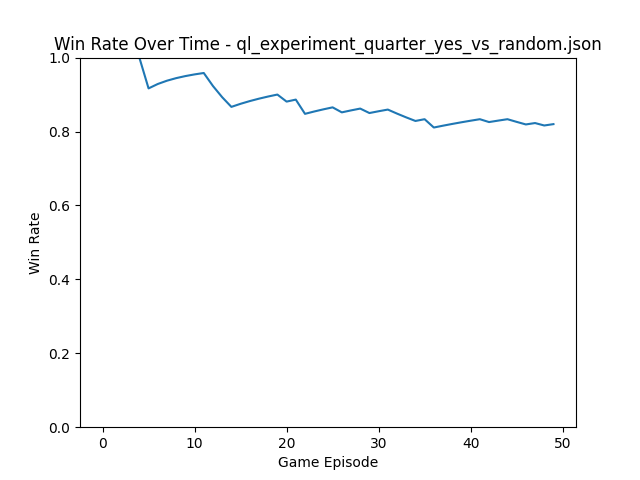
\includegraphics[width=0.25\textwidth]{images/win_rate_ql_experiment_quarter_yes_vs_random.png} &
    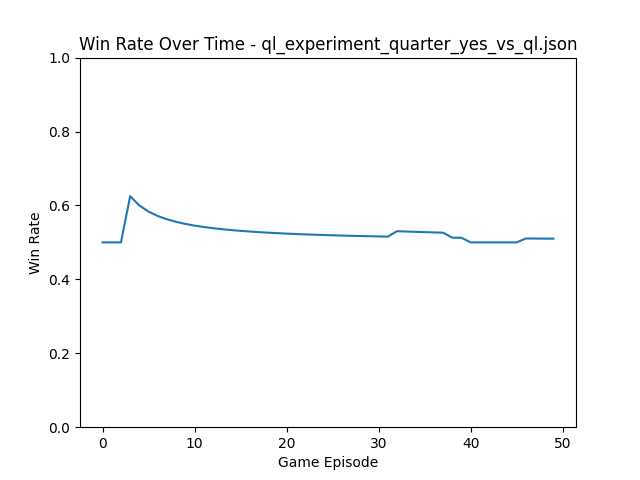
\includegraphics[width=0.25\textwidth]{images/win_rate_ql_experiment_quarter_yes_vs_ql.png} &
    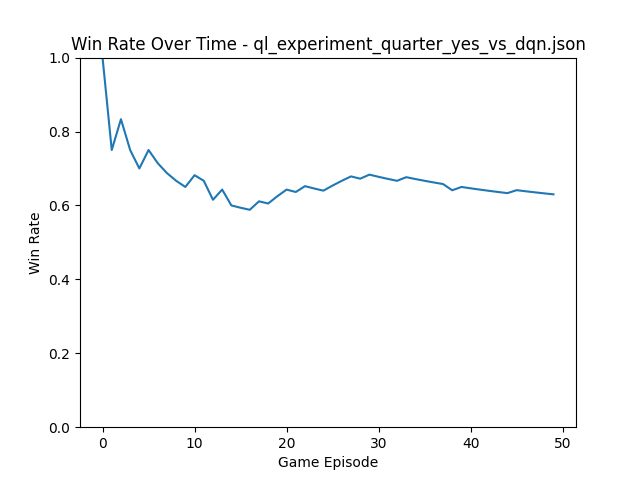
\includegraphics[width=0.25\textwidth]{images/win_rate_ql_experiment_quarter_yes_vs_dqn.png} \\
    \textbf{Second} & 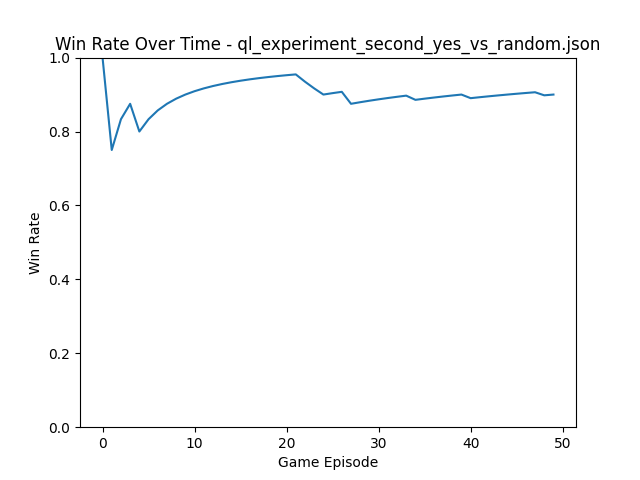
\includegraphics[width=0.25\textwidth]{images/win_rate_ql_experiment_second_yes_vs_random.png} &
    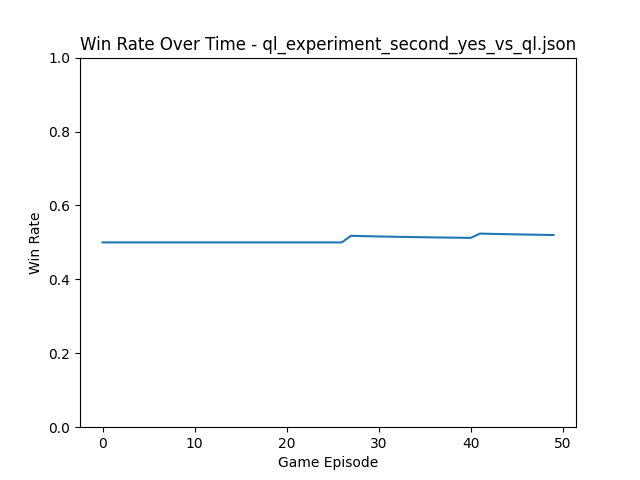
\includegraphics[width=0.25\textwidth]{images/win_rate_ql_experiment_second_yes_vs_ql.png} &
    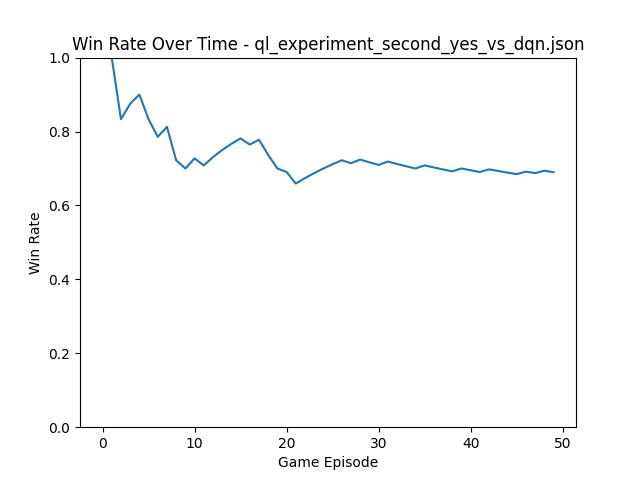
\includegraphics[width=0.25\textwidth]{images/win_rate_ql_experiment_second_yes_vs_dqn.png} \\
  \end{tabular}


There were a plethora of interesting results in this experiment. From DQN having several promising experiments showing the capability of maintaining around the same win ratio with every opponent, to the exact same experiment but with QL instead of DQN falling
completely flat and not able to compete at all. For DQN, neutral, quarter, and half without alternating seemed to maintain nearly the same win ratio across all of the models but second seems to perform better against the random agent but worse against the 
other two. Adding alternating into the equation seems to have the trained agent perform slightly better then without it but still maintained a similar win rate sitting at 50-60 percent. This could enable further research on developing agents that have 
differing degrees of challenging so that players can decide how much they want their skill to be pushed.

As for QL, the only option that showed any promise in without alternating was the neutral option, though maybe that is to be expected with the simplistic model. Throw in alternating into the model, and it still performs much to well against a lesser skilled 
opponent, the random agent, but is able to hit that around 50 percent goal for the other two. Not the most promising results with this model but still valuable data and there are definitely shortcomings that can be expanded upon in this experiment. 

  \subsection{Improvements}

How could future work or research build upon this experiment and overcome the shortcomings? Well the first would be to expand the environment to more decisions. Starcraft II for example has no shortage of those, the environment would simply need to have 
other possible actions and states added. Then the experiment could truly thrive when instead of 21 states and 6 actions, there could be thousands of states and hundreds of actions, depending on how far further research goes, as there are plenty more 
states and actions in this environment as discussed in a previous section. 

Secondly, better models. Both of these trained models, QL and DQN, are at the end of the day simplistic and not the end goal. Previous research mentioned have improved models that are trained on replays rather then just learning as they play, trained on 
multiple gpus rather then a single, consumer grade gpu, and trained over the course of weeks instead of days. This research in combination with those excellent papers and codebase seen before would induce a sophisticate experiment that will expand upon 
what was discovered here and give results that not just Starcraft II can do, but any games leading to possibly completely novel experience in games that has not been implemented yet. These improvements would be a few options of a path forward.